% Template per tesi di laurea
%
% Creato da Giulio Spinozzi
% giuliospinozzi@gmail.com
% http://giuliospinozzi.altervista.org
%
\documentclass [11pt,a4paper,oneside,openany]{book} %Classe del documento, formato carta, singola facciata, apertura capitoli pag destra/sinista (ininfluente se impostato oneside). Formato libro
\usepackage[italian]{babel} %Lingua Documento (da impostare per la sillabazione)
\usepackage{graphicx} %Pacchetto necessario per la gestione delle immagini
\usepackage{fancyhdr} %Pacchetto per la gestione accurata della pagina
\usepackage{setspace} %Pacchetto necessario per i comandi successivi onehalfspacing, singlespacing....
\usepackage{longtable} %Pacchetto per la gestione delle tabelle grandi
\usepackage[colorlinks=true]{hyperref} %Segnalibri nel pdf finale, sotto relativi parametri
\hypersetup{
	bookmarksnumbered=true,
	linkcolor=black,
	citecolor=black,
	urlcolor=black,
}

\usepackage{geometry} % Dimensione pagina
\geometry{a4paper} % Formato carta
\addtolength{\textheight}{75pt} %Margini
\oddsidemargin 30pt

\usepackage[latin1]{inputenc}
\usepackage{booktabs}
\usepackage{tabularx}
\usepackage{array}
\usepackage{url}
\usepackage{subfigure}
\usepackage{cite}
\usepackage{multirow}


\begin{document} %Inizio Documento

%%FRONTESPIZIO%%=========================================
\begin{titlepage}
 \begin{center}
     
\includegraphics[width=6cm]{img/logo.png}\\ %Logo dell'Universit� , cambiare il percorso, se necessario
     \vspace{1em}
     {\Large \textsc{Universit� degli studi di Perugia}}\\
     \vspace{1em}
     {\Large \textsc{Facolt� di Ingegneria}}\\
     \vspace{2em}
     {\normalsize Tesi di Laurea in}\\
     \vspace{1em}
     {\Large \textsc{Ingegneria Informatica e dell'Automazione}}\\
     \vspace{8em}
     {\LARGE \textbf{Generazione automatica di Word Cloud dinamiche}}\\
 \end{center}
 
 \vskip 2.5cm
  \begin{center}
    \begin{tabular}{c c c c c c c c}
      Relatore & & & & & & & Candidato \\[0.2cm]
      \Large{\textit{Prof. Carla Binucci}} & & & & & & & \Large{\textit{Enrico Spataro}}\\[0.4cm]
      Co-relatore & & & & & & & \\[0.2cm]
\Large{\textit{Prof. Walter Didimo}}  
    \end{tabular}
  \end{center}

\vskip 2.5cm
\begin{center}
{\normalsize Anno Accademico 2014/2015}
\end{center}
\end{titlepage}

%%DEDICA%%=============================================
\pagestyle{empty}
\vspace{5em}
\begin{flushright}
{\Large \textit{EVENTUALE DEDICA}}
\end{flushright}

\newpage

%%INTESTAZIONI PAGINA%%====================================
\pagestyle{fancy}
\renewcommand{\chaptermark} [1]{\chaptername\ \thechapter.\ #1}{} 
\renewcommand{\chaptermark}[1]{\markboth{\thechapter.\ #1}{}} 
\renewcommand{\sectionmark}[1]{\markright{\thesection\ #1}}
\fancyhf{}
\fancyhead[LE,RO]{\bfseries\thepage} 
\fancyhead[LO,RE]{\bfseries\leftmark} 
\fancypagestyle{plain}{%
\fancyhead{} % leva l'intestazione
\renewcommand{\headrulewidth}{0pt} % e la linea
}


%%INDICE%%==============================================
\tableofcontents
\listoffigures
\listoftables

%%CAPITOLI===============================================
\onehalfspacing

%%CAPITOLO 1: Introduzione=======================================
\chapter{Introduzione}

%%Scrivere normalmente, SENZA inserire begin e end document, che sono gi� compresi nel file principale da compilare

%%Il nostro lavoro � invece in direzione di quello che � il trend degli ultimi tempi, cio� quello di creare word cloud semantiche, in cui la disposizione delle parole riflette la loro correlazione semantica. %nome del file LaTeX del capitolo
\onehalfspacing

%%CAPITOLO 2: =======================================

\chapter{Word cloud statiche}

Questo capitolo consiste in una breve introduzione al concetto di word cloud.

Nel paragrafo \ref{wc_stat:def} verranno introdotte alcune definizioni e si parler� brevemente di qualche applicazione, mentre nel paragrafo \ref{wc_stat:sem} si far� il punto sullo stato dell'arte riguardo le word cloud semantiche.

\section{Definizioni e applicazioni}\label{wc_stat:def}
\subsection{Cos'� una word cloud?}
Il recente sviluppo di Internet, con l'avvento del Web 2.0, assieme al grande progresso tecnologico dei calcolatori, ha comportato un'ingente produzione di dati sul web e sulle piattaforme web based, per cui il problema di estrarre, gestire e visualizzare efficacemente tale informazione � diventata, negli ultimi anni, un'area di ricerca piuttosto importante nella visualizzazione dell'informazione. 

In generale, una \textbf{word cloud} � una rappresentazione visuale di documenti testuali, che utilizza diversi colori, font e dimensioni per raffigurare le parole pi� rilevanti, dette \textbf{keywords}, di un generico documento. Esse sono utilizzate, quindi, per esaminare un testo, in modo da facilitarne la comprensione, o per confrontare pi� testi. Ad esempio, nelle elezioni presidenziali del 2008 e del 2012 (fig. \ref{fig:obama_romney}), i media americani hanno confrontato le word cloud generate dai dibattiti dei candidati alla presidenza americana, mettendo in risalto le differenze tra i discorsi dei candidati; anche in Italia, in occasione del discorso di insediamento alla Camera da parte del presidente Mattarella, alcune testate giornalistiche hanno fatto uso delle word cloud per analizzare il contenuto del discorso. 
\begin{figure}
\centering
\subfigure[Word cloud generata dal discorso di Obama.]
{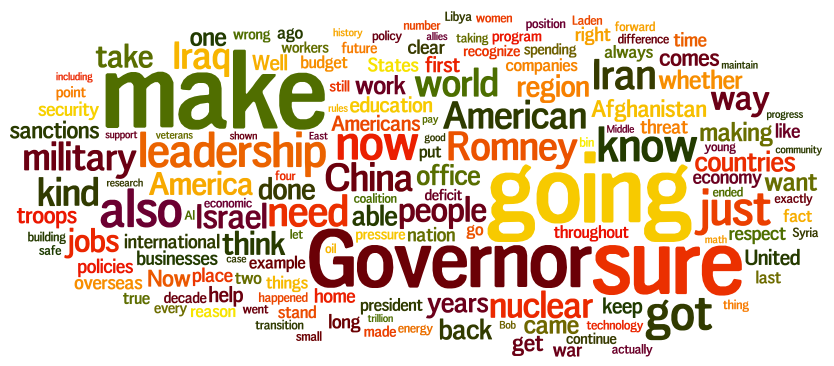
\includegraphics[scale=0.5]{img/wc_statiche/obama_wc.png}}
\hspace{3mm}
\subfigure[Word cloud generata dal discorso di Romney.]
{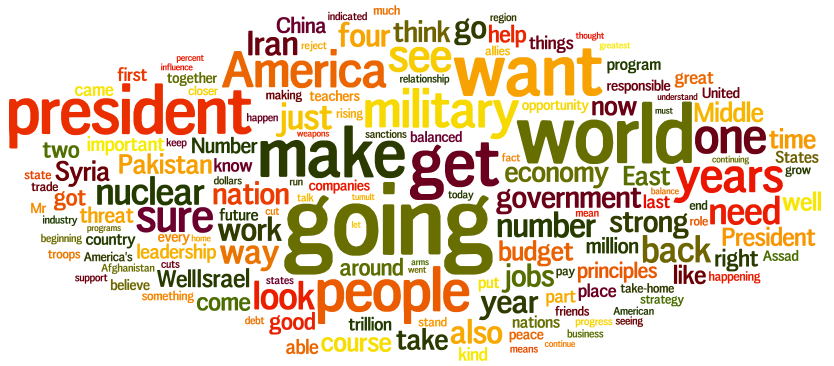
\includegraphics[scale=0.5]{img/wc_statiche/romney_wc.png}}
\caption[Due word cloud relative ai dibattiti tra i candidati alla presidenza statunitense.]{Due wordcloud relative ai dibattiti tra i candidati alla presidenza statunitense.}
\label{fig:obama_romney}
\end{figure}

In riferimento al web, si parla invece di \textbf{tag cloud}, con evidente richiamo ai tag, ovvero ai metadati che riassumono il contenuto di un sito internet. Ogni tag, rappresenta un link ad una specifica risorsa sul web, consentendo agli utenti di accedervi tramite l'utilizzo di keywords. Il loro utilizzo si � diffuso grazie al sito di \textit{photo sharing} Flickr\cite{flickr}, in cui i tag classificano in diverse categorie le foto che vengono condivise tra gli utenti.

Le parole di una word cloud sono tipicamente pesate in base all'importanza che esse ricoprono nel testo: pi� le parole hanno un font grande, pi� sono rilevanti. In questo modo, le word cloud permettono immediatamente di evidenziare ci� che � rilevante in un testo. Ci sono anche altri parametri da tenere in considerazione. In \cite{halvey}, Halvey et al. hanno valutato l'effetto di alcuni fattori: la posizione delle parole, la loro disposizione secondo l'ordine alfabetico e, come detto, la dimensione del font, si sono rivelati essere parametri importanti. Inoltre, hanno notato che gli utenti, piuttosto che leggere tutte le parole, danno uno sguardo generale alla word cloud. In un altro lavoro, Lohmann et al.\cite{Lohmann} hanno scoperto che parole posizionate vicino al centro catturano di pi� l'attenzione rispetto a parole vicine ai bordi, cos� come parole posizionate in alto a sinistra vengono percepite prima delle altre da parte degli utenti.

\subsection{Applicazioni}
Esistono diversi strumenti per la creazione di word cloud. Un tool web based molto popolare, Wordle\cite{Viegas:2009}, grazie alle qualit� grafiche e alle sue funzionalit�, ha permesso la diffusione delle word cloud come potente strumento per riassumere e analizzare un testo. Con Wordle, ad esempio, � possibile impostare alcuni parametri in modo da personalizzare la word cloud finale, come il numero delle parole, il colore, gli angoli di disegno ecc.. Tuttavia, Wordle non riesce a catturare le relazioni semantiche tra le parole, propriet� che pu� rivelarsi cruciale nell'analisi e nella comprensione di un testo. 
Per ovviare a ci�, � stato proposto un ulteriore strumento, basato su Wordle, chiamato ManiWordle\cite{kohk}, il quale offre un buon livello di interazione con l'utente, permettendo a quest'ultimo di manipolare il disegno finale e di modificare le parole visualizzate in termini di posizione, colore e orientamento, risultando quindi pi� flessibile di Wordle. Un altro sistema, SparkClouds\cite{lee}, tramite l'uso delle \textit{sparklines}, mette in risalto i cambiamenti tra pi� word cloud. Collins et al.\cite{collins}, hanno presentato Parallel Tag Clouds, uno strumento in grado di visualizzare le differenze tra i testi scritti di un ricco dataset. FacetAtlas\cite{facetatlas}, invece, � un'applicazione che, tramite grafici e mappe di densit�, visualizza le relazioni che intercorrono tra i documenti di una vasta collezione di testi.

In generale, dunque, negli anni, sono state sviluppate varie applicazioni che generano word cloud, ognuna con pregi e difetti, le quali permettono di comparare diversi documenti da pi� prospettive. Il nostro lavoro � in direzione di quello che � il trend degli ultimi tempi, cio� quello di creare word cloud semantiche, in cui la disposizione delle parole riflette la loro correlazione semantica.

\section{Word cloud semantiche}\label{wc_stat:sem}
Recentemente, la maggior parte dei tool che generano word cloud si � posta come obiettivo quello di raggruppare semanticamente le parole estratte, utilizzando tecniche di elaborazione del linguaggio naturale per correlare parole simili tra loro. Infatti, la possibilit� di disegnare, vicine nella word cloud, parole correlate semanticamente, pu� migliorare l'esperienza dell'utente, come notato da Deutsch et al. in \cite{Deutsch}.

Tree Cloud\cite{gambette}, ad esempio, � un applicazione in cui le parole vengono disposte secondo un albero, in modo tale da preservare la loro vicinanza semantica. In \cite{cui}, Cui et al., tramite misure di similarit�, mirano a collocare, vicine nel disegno, parole correlate semanticamente, utilizzando poi un metodo force directed per compattare la word cloud. Wu et al.\cite{seam}, utilizzano una tecnica ispirata al \textit{seam carving} per ottenere una word cloud semantica e compatta. Questo lavoro di tesi, invece, prende spunto dal recente lavoro svolto da Kobourov et al.\cite{kobourov}, in cui vengono implementati due nuovi algoritmi di visualizzazione, da confrontare con altri algoritmi esistenti, per analizzare la qualit� delle word cloud in base a diverse metriche, ovviamente partendo dalla base comune costituita dalla coerenza semantica nella disposizione delle parole. 
\onehalfspacing

%%CAPITOLO 3: =======================================

\chapter{Word cloud dinamiche}
Il concetto di word cloud dinamica, che � l'obiettivo di questa tesi, � descritto, dal punto di vista algoritmico, nel seguente capitolo. 
\\ \\
La sezione \ref{wc_din:def} offre una visione generale sul concetto di word cloud dinamica (cio� tempo variante), sullo stato dell'arte e alcuni cenni sui possibili contesti d'uso. Il paragrafo \ref{wc_din:algs} espone, fase per fase, il processo che consente di creare una word cloud statica da un testo di input, tenendo ben presente il vincolo di vicinanza semantica tra parole simili. Ogni fase � composta da diversi algoritmi, che vengono descritti progressivamente. Il capitolo quindi si chiude con la sezione \ref{wc_din:din_algs}, che presenta i passaggi necessari ad ottenere dinamicit� nel layout finale.

\section{Definizioni e applicazioni}\label{wc_din:def}
\subsection{Word cloud dinamiche e stato dell'arte}
Negli ultimi anni, sono state proposte diverse applicazioni per la creazione di word cloud. Oltre alla distinzione tra word cloud semantiche e non semantiche, � possibile suddividere tali applicazioni sulla base di due ulteriori categorie: word cloud \textbf{statiche} e word cloud \textbf{dinamiche} (o \textbf{tempo varianti}). La principale differenza tra queste due classi � chiaramente costituita dal fattore tempo: le word cloud dinamiche, infatti, hanno come obiettivo quello di illustrare l'evoluzione temporale di un documento o di un set di documenti. I grafici a barre, per esempio, sono tipicamente utilizzati per rappresentare l'andamento temporale di una qualche variabile e consentirne l'analisi visuale\cite{byron}\cite{havre}; Dubinko et al.\cite{dubinko} hanno sviluppato un tool che mostra l'evoluzione dei tag in Flickr e che permette l'interazione con gli utenti. Un lavoro rilevante, che tiene conto dell'evoluzione semantica e temporale di un insieme di documenti � stato effettuato da Cui et al.\cite{cui}: essi hanno proposto un sistema che abbina un grafico di tendenza (\textit{trend chart}) alle word cloud ottenute da documenti appartenenti ad una collezione. 

Sebbene tutti questi lavori abbiano come finalit� quella di visualizzare l'andamento temporale di un insieme di testi scritti, le informazioni spaziali e temporali sono rappresentate da immagini statiche. Diversamente, un lavoro interessante � stato svolto di recente da Chi et al.\cite{chi}, in cui viene mostrato il progresso temporale di un set di documenti tramite l'utilizzo di tecniche di \textit{morphing}\footnote{Il morphing consiste nella trasformazione fluida, graduale e senza soluzione di continuit� tra due immagini di forma diversa\cite{wiki:morphing}.}, che permettono di passare gradualmente da una word cloud di un documento ad un'altra di un altro documento, modificandone anche la forma (figura \ref{fig:morph_chi}). Tuttavia, come in\cite{cui}, la visualizzazione � relativa ad un insieme di documenti, quindi il periodo temporale preso in considerazione � piuttosto ampio. Inoltre, in questo studio, non viene affrontato l'aspetto semantico nei layout di ogni word cloud.  
\begin{figure}
\centering
{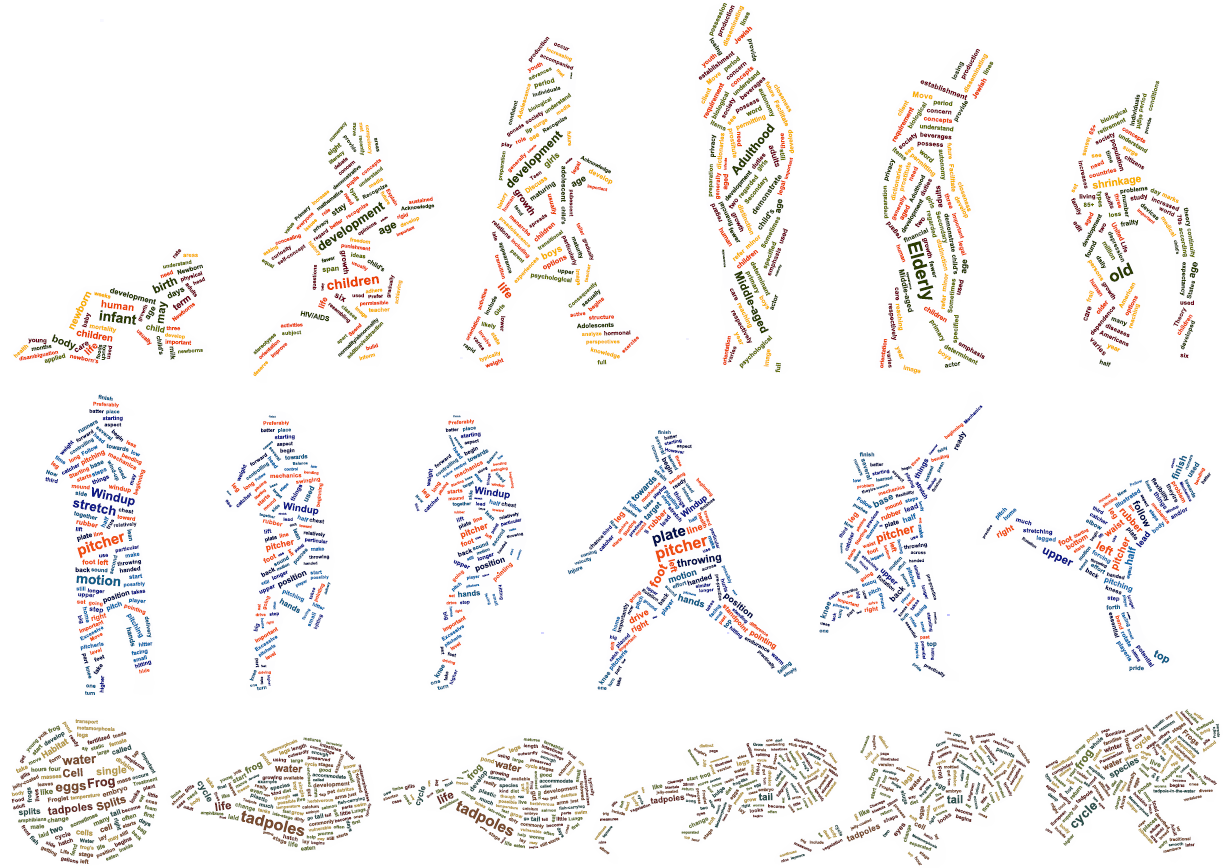
\includegraphics[scale=0.55]{img/wc_dinamiche/morphing_wc.png}}
\caption[Evoluzione di diverse word word cloud tramite tecniche di morphing.]{Evoluzione di diverse word word cloud tramite tecniche di morphing\cite{chi}: in alto, � mostrato il ciclo di vita dell'uomo; in mezzo, sono illustrati i movimenti effettuati dal pitcher nel baseball; in basso, infine, � mostrato il ciclo di vita di una rana.}
\label{fig:morph_chi}
\end{figure}

Il nostro lavoro, invece, a differenza degli altri citati precedentemente, si pone come finalit� quello di mostrare l'evoluzione di un solo testo, cio� il periodo temporale da cui si genera la word cloud � (relativamente) breve, poich� si prende in considerazione un solo documento. Per questo motivo, diventa significativo avere delle animazioni, che permettono di visualizzare l'evoluzione della word cloud insieme all'avanzamento dell'input. A tal fine, viene utilizzata una tecnica di morphing tra le word cloud generate in diversi istanti di tempo durante l'elaborazione del testo, rispettando, se possibile, il vincolo di vicinanza geometrica tra parole correlate semanticamente. Inoltre, � anche importante che non ci siano troppe differenze tra word cloud estratte in istanti successivi, ovvero parole che si muovono eccessivamente: l'utente potrebbe disorientarsi e perdersi durante l'evoluzione del testo, per cui la sua mappa mentale non deve cambiare in modo radicale. Da notare che, rispettare il vincolo di vicinanza semantica, insieme alla coerenza della mappa mentale, pu� costituire un compito impegnativo, dal momento che questi due vincoli costituiscono obiettivi contrastanti fra loro.
\subsection{Applicazioni}
I possibili utilizzi delle word cloud dinamiche, prodotte a partire da un unico testo di input, riguardano i contesti in cui si vuole visualizzare l'evoluzione di un generico documento relativo ad un breve periodo di tempo. Gli ambiti applicativi sono diversi, tra cui quello: 
\begin{itemize}
\item didattico, allo scopo, per esempio, di fornire uno strumento di ausilio nella comprensione di un testo;
\item divulgativo, per mostrare l'evoluzione di un discorso. Ci� pu� essere di grande utilit� per persone non udenti oppure nel caso di video riprodotti in luoghi con scarsa udibilit�; 
\item statistico, per illustrare l'evoluzione, in un breve periodo di tempo (ad esempio, in una giornata), dei trending topic dei vari social network;
\item ecc...
\end{itemize}

\section{Algoritmi di generazione di una word cloud semantica}\label{wc_din:algs}
Tutti gli algoritmi di visualizzazione di una word cloud ricevono in input un grafo pesato, i cui vertici sono le parole, rappresentate da rettangoli. Tuttavia, sono necessari alcuni passi di preprocessing, che consentono di estrarre questa informazione dall'input. L'algoritmo di visualizzazione disegna, per quanto possibile, le parole pi� simili vicine tra loro. Il processo di creazione di una word cloud � indicato in figura \ref{fig:pipeline}. Infine, viene applicato un algoritmo di clustering per assegnare lo stesso colore a parole dello stesso cluster.
\begin{figure}
\centering
{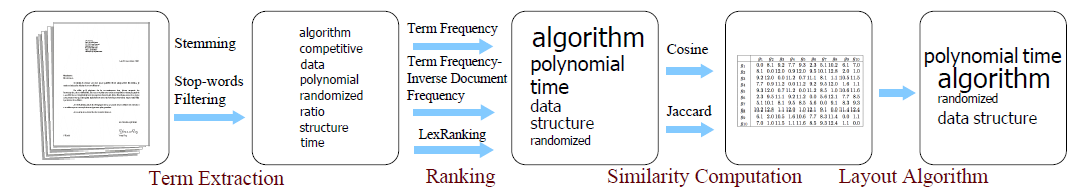
\includegraphics[scale=0.6]{img/wc_dinamiche/creation_steps.png}}
\caption[Generazione di una word cloud semantica.]{Generazione di una word cloud semantica.}
\label{fig:pipeline}
\end{figure}
\\ \\
Di seguito vengono prima esposti alcuni concetti teorici utilizzati nella definizione degli algoritmi. Successivamente, vengono descritte le varie fasi necessarie alla realizzazione di una word cloud semantica. 
\subsection{Riferimenti teorici}
\subsubsection{Grafo}
Un \textbf{grafo} $G$ � una coppia $(V,E)$, dove $V$ � un insieme finito ed $E$ � una relazione binaria in $V$. L'insieme $V$ � chiamato insieme dei vertici di $G$, mentre l'insieme $E$ � detto insieme degli archi di $G$. Un grafo si dice \textbf{orientato} se l'insieme degli archi $E$ � formato da coppie di vertici ordinate, altrimenti il grafo si dice \textbf{non orientato}. Dati due vertici $u,v \in V$, un arco che collega i due vertici � denotato con $(u,v)$ ed � detto \textbf{incidente} nei vertici $u$ e $v$. In tal caso, $u$ e $v$ sono gli \textbf{estremi} di $(u,v)$, e $u$ e $v$ sono \textbf{adiacenti}. Se un arco entra ed esce nello stesso vertice, allora si dice \textbf{cappio} (\textbf{self-loop}).

Dato un grafo $G=(V,E)$, si dice che $G'=(V'E')$ � un \textbf{sottografo} di $G$ se $V' \subseteq V$ ed $E' \subseteq E$. Dato un insieme $V' \subseteq V$, il sottografo di $G$ \textbf{indotto} da $V'$  � il grafo $G'=(V',E')$, dove $E' = \{(u,v) \in E : u,v \in V' \}$.
\subsubsection{Cammini e cicli}
Un \textbf{cammino} di lunghezza $k$ da un $u$ a $v$, con $u,v \in V$, in un grafo non orientato $G=(V,E)$, � una sequenza di vertici $(v_{0},v_{1},...,v_{k})$ tali che $u = v_{0}, v=v_{k}$ e $(v_{i-1},v_{i}) \in E$, con $0 \leq i \leq k$. La lunghezza del cammino � pari al numero di archi in $E$. \\
Un \textbf{ciclo} � un cammino $(v_{0},v_{1},...,v_{k})$ in cui $v_{0}=v_{k}$. Un cammino � \textbf{semplice} se tutti i suoi vertici sono distinti. Un ciclo � \textbf{semplice} se i vertici $(v_{0},v_{1},...,v_{k-1})$ sono distinti. Un cappio � un ciclo di lunghezza unitaria.

\subsubsection{Altre propriet� dei grafi}
Un grafo non orientato $G=(V,E)$ � \textbf{connesso} se ogni coppia di vertici � collegata attraverso un cammino, ovvero se ogni vertice � raggiungibile da ogni altro vertice. Le \textbf{componenti connesse} di un grafo $G$ sono i sottografi massimali connessi di $G$.

Un grafo non orientato � detto \textbf{aciclico} se non contiene cicli.  Un grafo non orientato e aciclico � una \textbf{foresta}; un grafo connesso, non orientato e aciclico � un \textbf{albero}. Si noti che ciascuna componente connessa di una foresta � un albero.

Un grafo non orientato si dice \textbf{bipartito} se l'insieme dei vertici $V$ pu� essere partizionato in due insiemi $U$ e $V$ tali che, se $(u,v) \in E$, allora $u \in U$ e $v \in V$ oppure $u \in V$ e $v \in U$. Un \textbf{matching} di $G$ � un insieme di archi tali che non ci sono due archi nell'insieme con un vertice in comune.
\subsection{Estrazione keywords}\label{wc_din:word_ext}
Il processo di estrazione delle keywords prevede una serie di passaggi preliminari, derivati da tecniche di elaborazione del linguaggio naturale, le quali predispongono, in maniera appropriata, il testo in ingresso all'algoritmo di estrazione delle parole.

Innanzitutto, il testo viene suddiviso in frasi. Poi, ogni sequenza di caratteri viene scomposta in \textit{token} (insiemi di caratteri, ad esempio parole, punteggiatura, numeri, simboli ecc...): ci� pu� essere eseguito mediante l'ausilio di librerie di elaborazione del linguaggio naturale (e.g. \textit{Apache OpenNLP}\cite{opennlp}). Successivamente, dal testo vengono eliminate le \textit{stop words}, cio� articoli, congiunzioni, parole di uso comune che sono poco rilevanti dal punto di vista informativo. Le parole rimanenti vengono quindi raggruppate in base alle rispettive radici (in inglese, \textit{stem}), tramite un algoritmo di \textit{stemming}: in questo modo, ad esempio, parole come \textit{play}, \textit{player}, \textit{played} e \textit{playing} vengono raggruppate secondo la radice comune \textit{play}. Nella nostra implementazione, � stato utilizzato il noto algoritmo \textbf{Porter Stemmer}\cite{porter}. Alla fine, nella word cloud finale, viene visualizzata la variante pi� frequente della parola.

Una volta eseguiti questi passaggi, si procede all'estrazione delle parole e al loro ranking in modo da trovare quelle pi� rilevanti, utilizzando tecniche di Information Retrieval. Ogni algoritmo assegna alle parole un punteggio e ne seleziona le $n$ pi� frequenti, dove $n$ � il numero di parole da visualizzare nella word cloud.
\\ \\
In questo lavoro di tesi sono state utilizzate diverse tecniche di estrazione delle keywords, qui di seguito esposte.
\subsubsection{Term Frequency (TF)}
Il modo pi� intuitivo di assegnare un peso alle parole consiste nel contare le loro singole occorrenze. Questo � ci� che viene fatto dall'algoritmo Term Frequency. Tuttavia, la rilevanza di un termine non aumenta linearmente con il numero delle occorrenze, in quanto documenti di una certa lunghezza potrebbero contribuire di pi� rispetto a documenti pi� corti, cio� potrebbero avere un peso maggiore nel conteggio delle occorrenze. Il calcolo della frequenza potrebbe quindi essere influenzato da questo fattore, per cui il punteggio di ogni parola spesso viene scalato tramite una qualche funzione. In tabella \ref{tab:tf}, sono riportate le tipiche funzioni che vengono utilizzate per pesare tale contributo (come indicato in \cite{manning}), dove l'argomento $ \textit{tf}_{t,d} $ indica la frequenza del termine $t$ nel documento $d$. 

\begin{table}[!htbp]
\centering
\renewcommand\arraystretch{1.4}
\begin{tabular}{|c|c|}
\hline
\textbf{Tipo funzione} &  \textbf{Peso} \\
\hline
Binaria & $0$,$1$ \\
\hline
Lineare & $ \textit{tf}_{t,d} $ \\
\hline
Radice quadrata & $ \sqrt{\textit{tf}_{t,d}} $ \\
\hline
Logaritmo & $ 1 + \log{\textit{tf}_{t,d}} $ \\
\hline
Doppia normalizzazione con parametro $K$ & $K + (1-K)* \frac{\textit{tf}_{t,d}}
{\max_{t' \in d} \textit{tf}_{t',d}}$ \\
\hline
\end{tabular}
\caption{Term Frequency ranking: funzioni}
\label{tab:tf}
\end{table}
Ad ogni modo, pur dopo aver rimosso le stop words, l'algoritmo Term Frequency tende ad assegnare punteggi troppo alti a termini poco rilevanti. Termini rari, invece, hanno contenuto informativo pi� alto rispetto a termini frequenti, per cui ad essi devono essere assegnati punteggi pi� elevati. In particolare, si definisce il parametro \textbf{IDF} (\textbf{Inverse Document Frequency}) di un termine $t$ la quantit�:
\begin{equation}
\textit{idf}_{t} = \log{\frac{N}{\textit{df}_{t}}},
\end{equation} 
dove $N$ � la dimensione di una collezione di documenti, mentre la quantit� $\textit{df}_{t}$ � detta \textit{document frequency}, che rappresenta il numero totale di documenti in cui il termine $t$ compare. Per termini frequenti in una collezione, tale valore tende a zero, mentre per termini meno frequenti il punteggio sar� pi� alto. Lo scaling che viene applicato � solitamente logaritmico, con qualche variante.

\subsubsection{TF-IDF}
Ora si possono combinare le due definizioni di TF e IDF per produrre un ulteriore algoritmo, noto come TF-IDF, il quale assegna, ad ogni termine $t$ di un documento $d$, la quantit�
\begin{equation}
\textit{tf-idf}_{t,d} = \textit{tf}_{t,d} \times \textit{idf}_{t}.
\end{equation}
Ne segue che:
\begin{itemize}
\item se $t$ � un termine comune nella collezione, avr� un $\textit{tf}_{t,d}$ alto, ma un $\textit{idf}_{t}$ vicino a zero, per cui $\textit{tf-idf}_{t,d}$ sar� tendente a zero;
\item se $t$ � un termine raro nella collezione, ma frequente nel documento $d$, allora avr� entrambi i contributi elevati, da cui ne deriva che $\textit{tf-idf}_{t,d}$ sar� alto.
\end{itemize} 
In pratica, con questo approccio, vengono filtrati i termini molto comuni, mentre quelli davvero rilevanti per il documento vengono estratti.

Uno degli schemi pi� noti in letteratura per calcolare la $\textit{tf-idf}_{t}$, come suggerito in \cite{manning} ed adottato in questa tesi, � il seguente:
\begin{equation}
\textit{tf-idf}_{t,d} = (1 + \log{\textit{tf}_{t,d}}) \times \log{\frac{N}{\textit{df}_{t}}}.
\end{equation}
\subsubsection{LexRank}
Il terzo algoritmo di ranking � LexRank\cite{lexrank}, gi� usato in \cite{seam} per la creazione di word cloud semantiche.  Tale algoritmo prende spunto da PageRank\cite{pagerank}, algoritmo utilizzato da Google per assegnare un punteggio alle pagine web e quindi migliorare le ricerche che si effettuano con il noto motore di ricerca.

LexRank � un algoritmo basato su un grafo $ G=(V,E) $, dove i vertici sono le parole, collegati da archi che rappresentano le co-occorrenze di due parole all'interno di una frase. Ogni arco $(i,j)$ ha infatti un peso $w_{ij}$, pari al numero di occorrenze della parola $i$ e della parola $j$ all'interno di una stessa frase. I punteggi vengono poi calcolati sfruttando il concetto di centralit� dell'autovettore definito da $G$. Tale valore di centralit� viene distribuito, da ogni vertice, ai suoi vicini. \\ Sia quindi $R$ il vettore di ranking, di dimensione $1 \times \vert V \vert$, dove $\vert V \vert$ � il numero dei nodi di $G$. Possiamo definire (per approfondimenti, consultare \cite{lexrank})
\begin{equation}
R = dM \cdot R + (1-d)p
\end{equation}
\begin{equation}
P \cdot R = \lambda R
\end{equation}
\begin{equation}
P = dM + (1-d)p \cdot 1^T
\end{equation}
dove:
\begin{itemize}
\item $d$ � il \textit{damping factor}, tipicamente scelto nell'intervallo $[0.1,0.2]$, come suggerito in \cite{lexrank};
\item $M$ � la matrice delle co-occorrenze normalizzata, avente dimensioni $\vert V \vert \times \vert V \vert$ e tale che la somma di ogni colonna sia pari a 1;
\item $p$ � il vettore delle probabilit�, di dimensione $1 \times \vert V \vert$, con ogni elemento pari a $1/\vert V \vert$;
\item $R$ � l'autovettore corrispondente al pi� grande autovalore di $M$ e pu� essere ricavato tramite l'algoritmo \textit{Power Method}, usato in \cite{lexrank}.
\end{itemize}
Alla fine, le parole estratte saranno costituite dai primi $n$ valori di $R$.

\subsection{Calcolo similarit�}\label{par:simil}
Il passo successivo � quello di calcolare la similarit� tra le keywords, ovvero quanto esse sono correlate tra loro. Data la lista delle $n$ parole estratte, viene calcolata la matrice $n \times n$ delle similarit� tra coppie di parole. Ogni valore � compreso tra 0 (nessuna correlazione) e 1 (massima correlazione). Esistono diversi algoritmi per il calcolo delle similarit�. Tutti usano uno spazio vettoriale di dimensione $n$ (pari al numero di parole estratte), dove il generico vettore $w_{i} = \{w_{i1},w_{i2},...,w_{in}\}$ rappresenta la co-occorrenza della $i$-esima parola con le altre $n-1$ parole. 
\\ \\ 
Di seguito sono esposte le tecniche di calcolo da noi implementate.

\subsubsection{Cosine Similarity}
La cosine similarity tra due vettori $w_{i}$ e $w_{j}$ viene calcolata come:
\begin{equation}
sim_{ij} = \frac{w_{i} \cdot w_{j}}{\vert\vert w_{i} \vert\vert \, \vert\vert w_{j} \vert\vert}
\end{equation}
In pratica, tale quantit� corrisponde alla misura dell'angolo formato tra i vettori $w_{i}$ e $w_{j}$. Se la similarit� � 1, allora l'angolo formato � pari $0�$, mentre se la similarit� � 0, allora i due vettori sono perpendicolari (angolo di intersezione $90�$) e non condividono alcuna frase.

\subsubsection{Jaccard Similarity}
La Jaccard similarity � definita come il rapporto tra il numero delle frasi condivise tra due parole e il numero totale delle frasi in cui esse compaiono. In formule:
\begin{equation}
sim_{ij} = \frac{\vert S_{i} \cap S_{j} \vert}{\vert S_{i} \cup S_{j} \vert},
\end{equation}
dove $S_{i}$ e $S_{j}$ sono, rispettivamente, l'insieme delle frasi in cui compare la parola $i$ e l'insieme delle frasi in cui compare la parola $j$.

\subsubsection{Jaccard Similarity estesa}
Un ulteriore modo per il calcolo della similarit� � rappresentato dalla Jaccard similarity estesa (anche nota come \textbf{coefficiente di Tanimoto}), definita come:
\begin{equation}
sim_{ij} = \frac{w_{i} \cdot w_{j}}{\vert\vert w_{i} \vert\vert^2 + \vert\vert w_{j} \vert\vert^2 - w_{i} \cdot w_{j}}
\end{equation}
Tale misura si riduce alla Jaccard Similarity nel caso di vettori binari.

\subsection{Creazione word cloud}
Gli algoritmi che producono word cloud ricevono in input una collezione di $n$ rettangoli (detti \textit{bounding box}), corrispondenti alle $n$ parole estratte, ognuno dei quali avente dimensioni proporzionali alla rilevanza della parola, e la matrice delle similarit� (di dimensione $n \times n$), dove ogni elemento � in $[0,1]$. L'output � costituito da un insieme di rettangoli sul piano e non sovrapposti. All'interno dei rettangoli sono disegnate le parole. Ovviamente, nel layout finale, saranno visibili solo le parole.
\\ \\
In questo lavoro di tesi sono stati utilizzati tre algoritmi: Context-Preserving Word Cloud Visualization\cite{cui}, Star Forest\cite{kobourov} e Cycle Cover\cite{kobourov}. Tutti e tre gli algoritmi sono stati pensati per una visualizzazione statica della word cloud, per cui essi sono stati modificati per tener conto dell'aspetto dinamico (pi� tardi vedremo come).

\subsubsection{Context-Preserving Word Cloud Visualization (CPWCV)}
Questo algoritmo, introdotto da Cui et al. in\cite{cui}, mira a soddisfare il vincolo di vicinanza geometrica tra parole correlate semanticamente in due passi: prima di tutto, viene calcolata, a partire dal contributo di ogni elemento $sim_{i,j}$ della matrice di similarit�, la distanza tra coppie di parole, pari a $d_{i,j}=1-sim_{i,j}$. Tale valore corrisponde alla distanza ideale tra la generica coppia di parole $(i,j)$ in uno spazio $n$-dimensionale. Viene quindi applicato uno \textit{scaling multidimensionale} (MDS), in modo da ottenere, su uno spazio bidimensionale, una prima collocazione delle parole tale da rispettare, approssimativamente, le distanze calcolate. Per preservare il posizionamento relativo tra le parole, si utilizza la \textit{triangolazione di Delaunay}\cite{delaunay}. Ci� crea un layout iniziale con occupazione dello spazio non ottimale. Perci� si applica un algoritmo force directed, che aggiorna le posizione delle parole mantenendo invariata la topologia del grafo, ovvero le relazioni semantiche tra le parole. Tale algoritmo si basa su tre principi:
\begin{itemize}
\item Principio di compattazione: questo principio mira a rimuovere, per quanto possibile, gli spazi tra le parole, in modo da ottenere un layout compatto;
\item Principio di non sovrapposizione: questa condizione richiede che le parole non siano sovrapposte, propriet� fondamentale per la leggibilit� della word cloud;
\item Principio di planarit�: per mantenere le relazioni semantiche tra le parole, il grafo � bene che sia planare, anche se ci� non � strettamente necessario. Inoltre imporre questa condizione pu� portare ad uno spreco di spazio.
\end{itemize}
Seguendo tali principi, la word cloud che si ottiene � compatta, facilmente leggibile e semanticamente coerente. Ognuna di queste propriet� � ottenibile applicando, rispettivamente, una forza elastica, una forza repulsiva e una forza attrattiva.

\subsubsection{Star Forest}
Introdotto in\cite{kobourov} da Kobourov et. al, Star Forest consiste in una \textbf{foresta di stelle}. Una foresta di stelle � una foresta dove le componenti connesse sono costituite da stelle. Una \textbf{stella} � un albero di profondit� massima pari a 1. 
\\ \\
L'algoritmo � composto da una sequenza di tre passaggi fondamentali:
\begin{enumerate}
\item Partizionamento del grafo, in modo da ottenere una foresta di stelle.
\item Applicazione dello scaling multidimensionale alla matrice delle distanze, ottenuta da quella delle similarit� tra coppie di parole, con conseguente creazione della word cloud per ogni stella.
\item Compattazione delle singole word cloud realizzate, da cui ne deriva il risultato finale.
\end{enumerate}
Le stelle vengono estratte dal grafo in modo \textit{greedy}. Si cerca un vertice $v$ i cui vertici adiacenti abbiano peso massimo, cio� tali che la somma $ \sum\nolimits_{u \in V} sim(u,v) $ sia massima. Si assume dunque che il vertice $v$ sia il centro della stella, mentre l'insieme dei vertici $V - \{v\}$ forma l'insieme delle foglie. Vengono scelte le parole adiacenti a $v$ e tali parole vengono rimosse dal grafo. Si ripete la procedura con grafi via via pi� piccoli, finch� non ci saranno pi� vertici.

\begin{figure}
\centering
{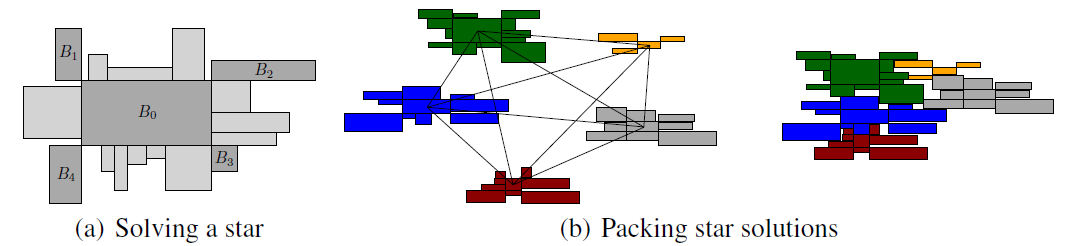
\includegraphics[scale=0.6]{img/wc_dinamiche/starforest.png}}
\caption[Algoritmo Star Forest.]{Algoritmo Star Forest.}
\label{fig:starforest}
\end{figure}

Selezionare il miglior insieme di parole adiacenti al centro $v$ della stella � un problema equivalente al noto problema dello zaino (\textit{Knapsack Problem}): dati $N$ oggetti, ognuno avente un peso e un valore, si vuole scegliere l'insieme di oggetti di maggior valore da inserire in uno zaino avente peso massimo sopportato pari a $W$. Sia dunque $B_{0}$ il bounding box corrispondente al centro della stella. In ogni soluzione ottima, ci sono quattro bounding box $B_{1},B_{2},B_{3},B_{4}$, ognuno avente un lato che contiene uno degli angoli di $B_{0}$ (figura \ref{fig:starforest}(a)). Dati $B_{1},B_{2},B_{3},B_{4}$, il problema si riduce ad assegnare ad ogni box $B_{i}$ uno dei quattro lati di $B_{0}$. Questo problema � equivalente ad un'istanza del problema dello zaino: il peso del bounding box $B_{i}$ � proporzionale alle sue dimensioni, dove la sua base � moltiplicata per la base di $B_{0}$ e l'altezza � moltiplicata per l'altezza di $B_{0}$, mentre il valore � pari al peso dell'arco che collega $B_{0}$ a $B_{i}$. L'algoritmo viene eseguito, in senso orario, a partire dal lato superiore di $B_{0}$. Per risolvere le istanze del problema, si utilizza l'algoritmo di approssimazione in tempo polinomiale descritto in\cite{ibarra}.

Le soluzione ottenute per le singole stelle vengono dunque messe insieme in un layout compatto, senza sovrapposizioni tra le parole e nel quale le relazioni semantiche tra le parole sono preservate (figura \ref{fig:starforest}(b)). Per ogni coppia di stelle $s_{1},s_{2}$, si ottiene la similarit� media tra le parole di $s_{1}$ e $s_{2}$ come $ sim(s_{1},s_{2}) = 
\dfrac{\sum\nolimits_{u \in s_{1}} \sum\nolimits_{v \in s_{2}} sim(u,v)}{\vert s_{1} \vert \vert s_{2} \vert}$. Si utilizza dunque l'MDS, con la distanza ideale tra le coppie di stelle posta uguale a
$ k(1 - sim(s_{1},s_{2})) $, dove $k$ � un fattore di scala, ottenendo cos� un primo layout. Poi, per compattare il disegno, si applica un algoritmo force directed. Da notare che esso viene applicato sulle stelle, non sulle singole parole. Tale algoritmo fa uso di due forze: 
\begin{itemize}
\item attrattiva, per rimuovere gli spazi vuoti, uguale a 
$ k_{a}(1 -  sim(s_{1},s_{2}))\Delta l$, con $\Delta l$ pari alla minima distanza tra i centri delle due stelle;
\item repulsiva, per evitare sovrapposizioni tra le varie parole, pari a  
$ k_{r}min(\Delta x,\Delta y)$, dove $\Delta x$ ($\Delta y$) corrisponde alla larghezza (altezza) della regione di spazio in sovrapposizione.
\end{itemize} 
Come ogni algoritmo force directed, questo metodo aggiorna le posizioni delle stelle iterativamente.

\subsubsection{Cycle Cover}
Questo algoritmo � stato proposto, come Star Forest, da Kobourov et. al in\cite{kobourov}. Esso si basa sull'estrazione di un sottografo planare dal grafo $G=(V,E)$ definito dalla matrice di similarit�. Tale sottografo � composto da un insieme disgiunto di cicli di peso massimo ed � denominato, appunto, \textit{cycle cover}.

L'algoritmo che calcola il cycle cover estrae, dal grafo $G$, un grafo bipartito $H$. Si inizializza infatti $H$ con i vertici di $G$. Poi, per ogni $v \in V(G)$, si aggiunge un vertice $v' \in V(H)$, e per ogni arco $(u,v) \in E(G)$, vengono creati due archi, $(u',v)$ e $(u,v') \in E(H)$, aventi peso pari a $sim(u,v)$. Il grafo $H$ risultante � bipartito per costruzione ed � facile ricavare un matching di peso massimo. Tale matching consiste in un insieme di cammini e cicli disgiunti di $G$, in quanto ogni $u$ � accoppiato a $v'$ e ogni $u'$ � accoppiato a $v$.

\begin{figure}
\centering
{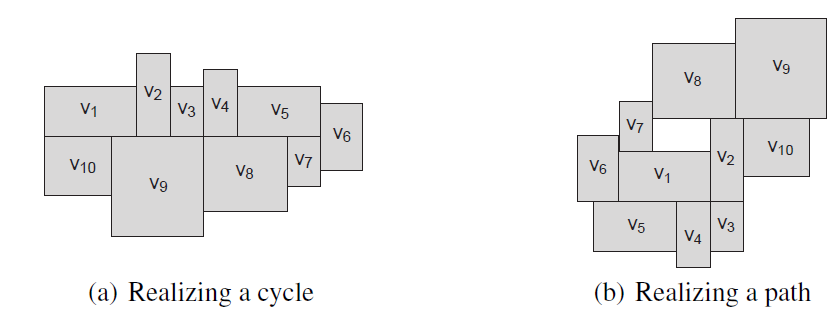
\includegraphics[scale=0.7]{img/wc_dinamiche/cyclecover.png}}
\caption[Algoritmo Cycle Cover.]{Algoritmo Cycle Cover.}
\label{fig:cyclecover}
\end{figure}

Fissato dunque un ciclo $(v_{1},v_{2},...,v_{n})$, sia $t$ il massimo indice  tale che $ \sum\nolimits_{i \leq t} w_{i} \leq \sum\nolimits_{i \leq n} w_{i}/2 $, dove $w_{i}$ � la base del bounding box corrispondente alla parola i-esima. I vertici $v_{1},v_{2},...,v_{t}$ vengono collocati orizzontalmente da sinistra verso destra, mentre i vertici $v_{n},v_{n-1},...,v_{t+2}$ vengono collocati da destra verso sinistra. In entrambi i casi, i vertici sono allineati su una stessa linea (figura \ref{fig:cyclecover}(a)). Rimane da piazzare il vertice $v_{t+1}$, in contatto tra $v_{t}$ e $v_{t+2}$. Si sceglie il gruppo di vertici (superiore o inferiore) i cui rettangoli hanno la minima larghezza oppure lo si pone a met� tra  $v_{t}$ e $v_{t+2}$. I cicli vengono convertiti in cammini se sono composti da pi� di 10 vertici. In tal caso, dopo aver posizionato i vertici $v_{1}$ e $v_{2}$ vicini l'un l'altro, si procede a piazzare il generico vertice $v_{i}$ in modo tale che tocchi $v_{i-1}$ nel primo spazio disponibile in senso orario, ottenendo cos� un layout a spirale.

Successivamente, cos� come nell'algoritmo Star Forest, le soluzioni individuali realizzate vengono messe insieme. Poi si applica lo stesso algoritmo force directed, descritto precedentemente, per compattare il disegno e rimuovere eventuali intersezioni tra le parole.

\subsection{Clustering}
Una volta ottenuto il layout, si prosegue con l'applicazione di un algoritmo di \textit{clustering}, il quale suddivide le parole in pi� gruppi (\textit{cluster}). Ad ogni cluster viene assegnato un colore diverso e ogni colore identifica un diverso raggruppamento semantico. In generale, l'obiettivo del clustering � quello di ottenere che gli oggetti di ogni cluster siano il pi� possibile simili tra loro, o comunque che la loro correlazione sia pi� alta rispetto a quella con oggetti di cluster diversi.
\\ \\
L'algoritmo di clustering utilizzato in questa tesi � K-means++, proposto da Arthur et. al in\cite{arthur}, ed � una versione migliorata di uno dei pi� noti algoritmi in letteratura, K-means. Prima verr� quindi presentato K-means, per poi passare alla variante K-means++.

\subsubsection{K-means}
K-means � un tipo di algoritmo \textbf{prototype-based}, cio� basato sul concetto di \textbf{prototipo}, che � l'elemento pi� rappresentativo di un cluster. Infatti, un cluster � una collezione di oggetti in cui ogni oggetto � pi� simile al prototipo del rispettivo cluster piuttosto che ai prototipi di altri cluster. K-means definisce il prototipo in termini di \textbf{centroide}, tipicamente inteso come elemento medio di un insieme di punti.

La tecnica di clustering definita dal K-means � piuttosto semplice e intuitiva, oltre ad essere veloce, sebbene non ci sono garanzie riguardo l'accuratezza del risultato. In generale, dato un intero $K>0$ e un insieme di $n$ oggetti di un dataset $\chi$, si vogliono scegliere $K$ centroidi, tali da minimizzare (o massimizzare) la funzione obiettivo 
\begin{equation}\label{kmeans_formula}
\phi = \sum\limits_{i=1}^K \sum\nolimits_{x \in C_{i}} dist(x,c_{i}),
\end{equation}
dove $C_{i}$ � l'i-esimo cluster e $dist(x,c_{i})$ � una qualche misura di prossimit� tra il generico elemento $x \in C_{i} $ e il centroide $c_{i}$ dell'i-esimo cluster. In pratica, ci� che si vuole ottenere, sono $k$ cluster in cui gli oggetti appartenenti ad ogni cluster siano il pi� possibile simili tra loro. 
\\ \\
L'ottimizzazione della funzione obiettivo � un problema NP-completo, per cui l'approccio comunemente adottato prevede le seguenti fasi, che fanno convergere l'algoritmo ad una soluzione locale (figura \ref{fig:kmeans_ex}): 
\begin{enumerate}
\item Si scelgono $K$ centroidi $C=\{c_{1},...,c_{k}\}$.
\item Ogni elemento $x \in \chi$ viene associato al centroide pi� vicino. Ogni collezione di elementi associata a $c_{i}, i \in \{1,...,k\}$, forma un cluster.
\item Si aggiorna il centroide di ogni cluster.
\item I passi 2 e 3 vengono eseguiti iterativamente finch� non si osservano ulteriori variazioni nell'insieme dei centroidi.
\end{enumerate}
\begin{figure}
\centering
{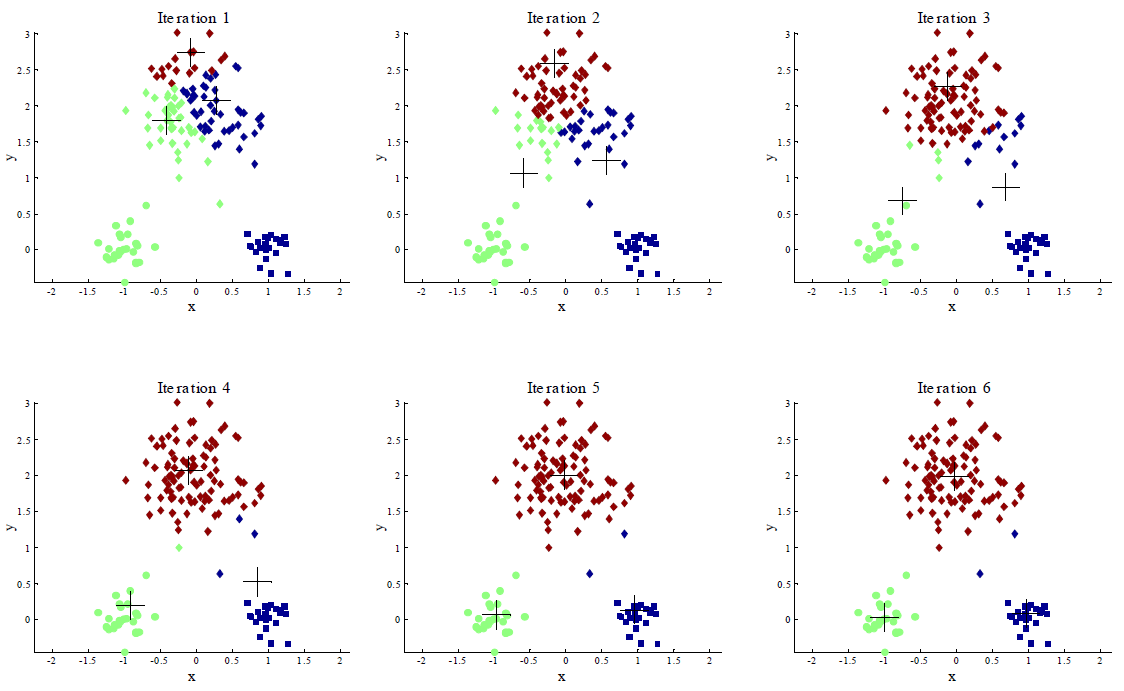
\includegraphics[scale=0.6]{img/wc_dinamiche/kmeans_ex.png}}
\caption[K-means: esempio di esecuzione dell'algoritmo. In questo caso si ottengono $K=3$ cluster.]{K-means: esempio di esecuzione dell'algoritmo\cite{tan}. In questo caso si ottengono $K=3$ cluster.}
\label{fig:kmeans_ex}
\end{figure}
Spesso i centroidi iniziali vengono selezionati in modo randomico, ma � possibile seguire diversi approcci. In ogni caso, supponendo di voler minimizzare la funzione obiettivo, l'idea dell'algoritmo � quella di decrementare, ad ogni esecuzione, il valore della funzione $\phi$, mediante i passi 2 e 3, finch� non vengono osservate variazioni nei centroidi. Infatti, $\phi$ � una funzione monotona decrescente, per cui ad ogni esecuzione il suo valore al massimo rimane invariato. Dal momento che ci sono $k^n$ raggruppamenti possibili, l'esecuzione dell'algoritmo termina sempre.

L'obiettivo dell'algoritmo, come detto, � quello di minimizzare (massimizzare) la funzione obiettivo $\phi$. Tale funzione, misura la qualit� del clustering tramite il calcolo della prossimit� (similarit�) tra il centroide $c_{i}$ e gli elementi del cluster $C_{i}$. Solitamente, i punti fanno parte di uno spazio $n$-dimensionale e come misura di prossimit� si utilizza la distanza euclidea. Ad ogni modo, ci sono diverse possibilit� per la scelta della misura di prossimit�, come indicato in tabella \ref{tab:prox_kmeans}\cite{tan}. 
\begin{table}[!htbp]
\centering
\renewcommand\arraystretch{1.4}
\begin{tabular}{|c|c|p{5cm}|}
\hline
\textbf{Funzione di prossimit�} &  \textbf{Centroide} & \textbf{Funzione obiettivo} \\
\hline
Manhattan & mediana & Minimizzare la somma delle distanze di ogni oggetto dal centroide del suo cluster \\
\hline
Euclidea & media & Minimizzare la somma delle distanze (al quadrato) di ogni oggetto dal centroide del suo cluster \\
\hline
Similarit� (coseno, Jaccard...) & media & Massimizzare (minimizzare) la similarit� (dissimilarit�) di ogni oggetto con il centroide del cluster di appartenenza  \\
\hline
Divergenza di Bregman & media & Minimizzare la somma della divergenza di Bregman di ogni oggetto con il centroide del cluster di appartenenza \\
\hline
\end{tabular}
\caption{K-means: scelte comuni per le misure di prossimit�.}
\label{tab:prox_kmeans}
\end{table}
\vspace{0.5cm}
\subsubsection{K-means\texorpdfstring{++}{}}
La differenza principale tra il K-means++ e il K-means classico consiste nell'inizializzazione dell'algoritmo, ovvero nella scelta dei $K$ centroidi iniziali, da cui dipende la qualit� del clustering finale. La fase di inizializzazione, infatti, consiste di diversi passaggi, di seguito esposti: 
\begin{enumerate}
\item Si sceglie il primo centroide $c_{1}$ in modo casuale tra tutti i punti (nel nostro caso le parole).
\item Per ogni altro elemento del dataset, $x \in \chi$, si calcola la distanza $dist(x,c_{i})$ tra $x$ e il centroide pi� vicino $c_{i}$ tra quelli gi� selezionati.
\item Un elemento generico $x$ pu� quindi diventare un centroide con probabilit� pari a $\dfrac{dist(x,c_{i})^2}{\sum\nolimits_{x \in \chi} dist(x,c_{i})^2} $.
\item Si ripetono gli step 2 e 3 finch� non si hanno $K$ centroidi.
\item Avendo ottenuto un insieme di $K$ centroidi, si pu� procedere con il K-means classico.
\end{enumerate}
Con l'inizializzazione suggerita dalla tecnica K-means++, l'algoritmo riesce a trovare una soluzione che � $O(log\;k)$-competitiva rispetto alla soluzione ottima fornita dal K-means classico. 

Per quanto riguarda l'applicazione dell'algoritmo al nostro lavoro, si parte da un dataset costituito dall'insieme delle $n$ parole $W=\{w_{1},...,w_{n}\}$, estratte in fase di pre-processing. Come misura di prossimit� � stata utilizzata la distanza semantica tra le parole ricavata dalla matrice di similarit�. Il clustering quindi non viene eseguito sul disegno finale, cio� in base al posizionamento sul piano delle parole, ma a partire dalla loro similarit�. Ne segue che il raggruppamento delle parole � logico, non geometrico (ovvero tramite la distanza euclidea, come spesso avviene). La funzione obiettivo da minimizzare diventa dunque 
\begin{equation}\label{kmeansplusplus_formula}
\phi = \sum\limits_{i=1}^K \sum\nolimits_{w \in C_{i}} (1 - sim_{w,c_{i}})
\end{equation}
\section{Algoritmi di generazione di una word cloud semantica e dinamica}\label{wc_din:din_algs}
Nel paragrafo precedente, � stata presentata la procedura, insieme agli algoritmi, necessaria a realizzare una word cloud semantica a partire da un testo in input. Tuttavia, tali algoritmi sono stati pensati per un singolo layout statico, cio� invariante nel tempo. L'obiettivo del nostro lavoro � invece quello di mostrare l'evoluzione della word cloud di un documento. A tal fine, vengono create diverse word cloud del testo ad intervalli regolari. Per passare da un layout al successivo in modo dinamico, � stata applicata una semplice tecnica di \textit{morphing}. La dinamicit�, come vedremo meglio dopo, dipende dallo stato delle parole, poich� esse possono apparire, scomparire o rimanere nel layout durante il passaggio da una word cloud ad un'altra. Ci� significa che bisogna tener conto di diversi aspetti: variazione della posizione delle parole, variazione delle dimensioni delle parole in base al punteggio via via ottenuto e variazione dei colori. Tuttavia, conferire dinamicit� comporta alcune problematiche: 
\begin{itemize}
\item le parole comuni a due successive word cloud potrebbero variare di molto le rispettive posizioni, disorientando l'utente e portando confusione alla sua mappa mentale;
\item i cluster pi� simili di due layout consecutivi devono poter mantenere lo stesso colore (quanti cluster manterranno il colore lo vedremo dopo).
\end{itemize}
Per la prima criticit�, sono stati modificati gli algoritmi di disegno: lo spostamento di una parola dipende dalla sua rilevanza, per cui parole importanti variano poco la propria posizione. Questo � un obiettivo discordante con il mantenimento delle relazioni semantiche tra le parole, per cui � necessario calibrare i parametri in base alle proprie esigenze.
\\ \\ 
Per il secondo problema, invece, sono stati applicati gli algoritmi per il calcolo della similarit� descritti in precedenza (vedi paragrafo \ref{par:simil}), cos� da accoppiare i cluster pi� simili in layout consecutivi (la similarit� � intesa come numero di parole in comune tra i vari cluster).
\\ \\
Nel seguito, verranno esposti i passaggi necessari a risolvere le due criticit� sopra elencate. Chiude la sezione la descrizione della tecnica di morphing utilizzata nel passaggio da una word cloud alla successiva.

\subsection{Creazione word cloud}
Gli algoritmi di disegno sono stati modificati come segue (eccetto ovviamente nella creazione del primo disegno): 
\begin{itemize}
\item fissate $K$ word cloud, siano $\Gamma^{k-1}$ e $\Gamma^{k}$ due disegni consecutivi, con l'intero $k \in \{2,...,K\}$;
\item consideriamo inoltre le $p$ parole che compaiono sia in $\Gamma^{k-1}$ che in $\Gamma^{k}$, cio� l'insieme $P = \{w_{1},...,w_{p}\}$. Per ogni $w_{i} \in P$, si denotano con $\tau_{i}^{k-1}$ la posizione di $w_{i}$ in $\Gamma^{k-1}$, con $\tau_{i}^{k}$ la posizione di $w_{i}$ in $\Gamma^{k}$ e con $ \rho_{i}^{k}$ il punteggio assegnato a $w_{i}$ in $\Gamma^{k}$ nella fase di estrazione delle parole;
\item una volta ottenuto, durante la realizzazione di $\Gamma^{k}$ con uno degli algoritmi di disegno descritti precedentemente, un layout iniziale con l'utilizzo dell'MDS, si applica un metodo force directed che, iterativamente, effettua una traslazione di $\tau_{i}^{k-1}$ in $\tau_{i}^{k}$. Questa traslazione � per� contrastata da $\rho_{i}^{k}$. La forza applicata dall'algoritmo durante la traslazione � dunque inversamente proporzionale a $\rho_{i}^{k}$, cio� $ f_{k-1,k} \propto 1/\rho_{i}^{k}$. 
\end{itemize} 
Cos� facendo, le parole pi� importanti tendono a non cambiare continuamente posizione e quindi la mappa mentale dell'utente non varia di molto. Ci� � significativo, poich� la word cloud dinamica di un solo testo deve essere intuitiva e non deve portare confusione all'utente, sebbene questo possa significare una perdita di prestazioni dal punto di vista della vicinanza semantica delle parole (le parole, infatti, possono cambiare cluster tra un disegno e l'altro).

\subsection{Calcolo similarit� tra cluster}
Per quanto riguarda la seconda criticit�, si procede al calcolo della similarit� tra cluster con uno degli algoritmi descritti in precedenza. La similarit�, praticamente, viene valutata sulla base di quante parole i cluster hanno in comune tra una word cloud e la successiva. 
\\ \\
Il procedimento adottato � il seguente:
\begin{itemize}
\item fissate $K$ word cloud, siano $\Gamma^{k-1}$ e $\Gamma^{k}$ due disegni consecutivi, con l'intero $k \in \{2,...,K\}$. 
\item denotiamo con $ C^{k-1} = \{c_{0}^{k-1},c_{1}^{k-1},...,c_{l}^{k-1}, \}$ e con $ C^{k} = \{c_{0}^{k},c_{1}^{k},...,c_{m}^{k}, \}$ gli insiemi dei cluster presenti rispettivamente in $\Gamma^{k-1}$ e in $\Gamma^{k}$, entrambi aventi dimensione $ l,m > 0 $. 
\item si esegue il calcolo della similarit� a coppie tra i due insiemi di cluster e la si indica con $ sim_{c_{i}^{k-1},c_{j}^{k}} $, dove $ i \in \{1,...,l\}$ e $ j \in \{1,...,m\}$. Le varie coppie ottenute vengono ordinate in ordine decrescente su una lista di dimensione $l \times m$. L'ordine � dato dal valore di similarit� di ciascuna coppia. 
\item data la prima coppia nella lista, ad esempio $(c_{a}^{k-1},c_{b}^{k})$, si associa $b$ ad $a$. In questo modo, il cluster $b$ avr� lo stesso colore di $a$. Vengono quindi eliminate tutte le occorrenze di $c_{a}^{k-1}$ e $c_{b}^{k}$ nella lista. Si procede cos� per tutte le altre coppie. 
\end{itemize}
Si noti che il numero totale di cluster che nella word cloud $\Gamma^{k}$ manterr� il colore � uguale a $min(l,m)$.

\subsection{Morphing tra successive word cloud}
Il morphing � stato applicato per gestire in modo fluido e continuo, tra una word cloud ed un'altra, il cambiamento di stato delle parole, cio� le variazioni di posizione e dimensione. Un approccio simile � stato usato anche a livello di interfaccia grafica per la gestione delle variazioni di colore delle parole.
\\ \\
Dati due disegni consecutivi $\Gamma^{k-1}$ e $\Gamma^{k}$, con $k \in \{2,...,K\}$, indichiamo con:
\begin{itemize}
\item $P = \{w_{1},...,w_{p}\}$ l'insieme delle parole comuni a $\Gamma^{k-1}$ e $\Gamma^{k}$;
\item $S = \{w_{1},...,w_{s}\}$ l'insieme delle parole in $\Gamma^{k-1}$ che non compaiono in $\Gamma^{k}$;
\item $C = \{w_{1},...,w_{c}\}$ l'insieme delle parole in $\Gamma^{k}$ che non compaiono in $\Gamma^{k-1}$;
\item $N$ il numero di frame tra un layout ed un altro (pi� $N$ � alto, pi� l'animazione � fluida).
\end{itemize}
La parola i-esima $w_{i}$ pu� far parte di tre diversi insiemi. A seconda dei casi, il comportamento pu� variare. Analizziamo ogni possibile situazione:
\begin{enumerate}
\item \textbf{$w_{i} \in C$}: poich� $w_{i}$ compare solo in $\Gamma^{k}$ con un punteggio pari a $\rho_{i}^{k}$, si pu� assumere che essa avr� un punteggio pari a 0 in $\Gamma^{k-1}$. Avendo $N$ frame compresi tra $\Gamma^{k-1}$ e $\Gamma^{k}$, il punteggio viene incrementato, ad ogni frame, di una quantit� pari a $\dfrac{\rho_{i}^{k}}{N+1}$. Di conseguenza, in base al punteggio corrente della parola, anche la dimensione del rispettivo bounding box viene opportunamente modificata ad ogni frame (vedi figura \ref{fig:new_word}).
\begin{figure}
\centering
{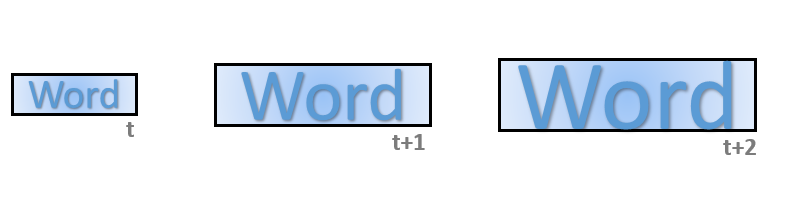
\includegraphics[scale=1]{img/wc_dinamiche/new_word.png}}
\caption[Esempio di parola che compare in $\Gamma^{k}$ ma non in $\Gamma^{k-1}$. In figura � illustrato lo stato della parola in 3 istanti consecutivi.]{Esempio di parola che compare in $\Gamma^{k}$ ma non in $\Gamma^{k-1}$. In figura � illustrato lo stato della parola in 3 istanti consecutivi.}
\label{fig:new_word}
\end{figure}
\item $w_{i} \in S$: caso opposto al precedente, ovvero $w_{i}$ compare solo in $\Gamma^{k-1}$ con un punteggio pari a $\rho_{i}^{k-1}$, per cui si assume che essa avr� un punteggio pari a 0 in $\Gamma^{k}$. Poich� tra $\Gamma^{k-1}$ e $\Gamma^{k}$ ci sono $N$ frame, il punteggio viene decrementato, ad ogni frame, di una quantit� pari a $\dfrac{\rho_{i}^{k-1}}{N+1}$. Come nel caso precedente, la dimensione del rispettivo bounding box viene opportunamente modificata ad ogni frame in base al punteggio corrente della parola (figura \ref{fig:disapp_word}).
\begin{figure}
\centering
{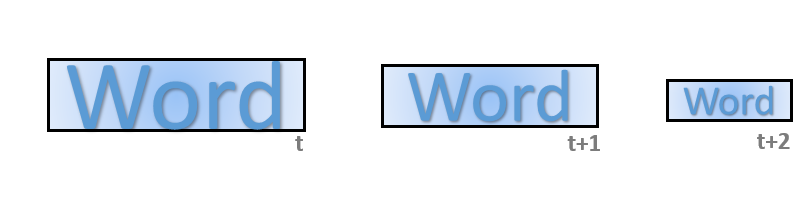
\includegraphics[scale=1]{img/wc_dinamiche/disapp_word.png}}
\caption[Esempio di parola che compare in $\Gamma^{k-1}$ ma non in $\Gamma^{k}$. In figura � illustrato lo stato della parola in 3 istanti consecutivi.]{Esempio di parola che compare in $\Gamma^{k-1}$ ma non in $\Gamma^{k}$. In figura � illustrato lo stato della parola in 3 istanti consecutivi.}
\label{fig:disapp_word}
\end{figure}
\item $w_{i} \in P$: � il caso pi� complesso dei tre. Il termine $w_{i}$ compare in entrambi i layout. Indicati con $\rho_{i}^{k-1}$ il punteggio di $w_{i}$ in $\Gamma^{k-1}$, con $\rho_{i}^{k}$ il punteggio di $w_{i}$ in $\Gamma^{k}$ e con $\Delta_{\rho_{i}}^{k,k-1} = \vert\rho_{i}^{k}-\rho_{i}^{k-1}\vert$ la differenza in valore assoluto tra i due punteggi, se:
\begin{itemize}
\item $\rho_{i}^{k} < \rho_{i}^{k-1} $, il peso di $w_{i}$ viene decrementato di $\dfrac{\Delta_{\rho_{i}}^{k,k-1}}{N+1}$ ad ogni frame;
\item $\rho_{i}^{k} > \rho_{i}^{k-1} $, il peso di $w_{i}$ viene incrementato di $\dfrac{\Delta_{\rho_{i}}^{k,k-1}}{N+1}$ ad ogni frame;
\end{itemize}
In base al punteggio corrente, ad ogni frame la dimensione del rispettivo bounding box di $w_{i}$ viene opportunamente aggiornata. Ovviamente, il peso rimane invariato nel caso in cui il punteggo non cambia tra un disegno e l'altro. \\ 
Inoltre, in questo caso, le parole vengono anche traslate, quindi le posizioni dei rispettivi bounding box variano. Siano dunque:
\begin{itemize}
\item $\tau_{i}^{k-1}=(x_{i}^{k-1},y_{i}^{k-1})$ il centro di $w_{i} $ in $\Gamma^{k-1}$;
\item  $\tau_{i}^{k}=(x_{i}^{k},y_{i}^{k})$ il centro di $w_{i} $ in $\Gamma^{k}$;
\item $\delta_{\tau_{i}}^{k,k-1} = \vert\vert \tau_{i}^{k} - \tau_{i}^{k-1} \vert\vert$ la distanza tra $\tau_{i}^{k}$ e $\tau_{i}^{k-1}$;
\end{itemize}
Ad ogni frame, il bounding box viene traslato, in valore assoluto, di una quantit� pari a $\dfrac{\delta_{\tau_{i}}^{k,k-1}}{N+1}$. La direzione dello spostamento dipende dal relativo posizionamento di $\tau_{i}^{k-1}$ in $\Gamma^{k-1}$ e di $\tau_{i}^{k}$ in $\Gamma^{k}$. Abbiamo in generale quattro casi diversi, come indicato in figura \ref{fig:morphcommon}.
\begin{figure}
\centering
\subfigure[]
{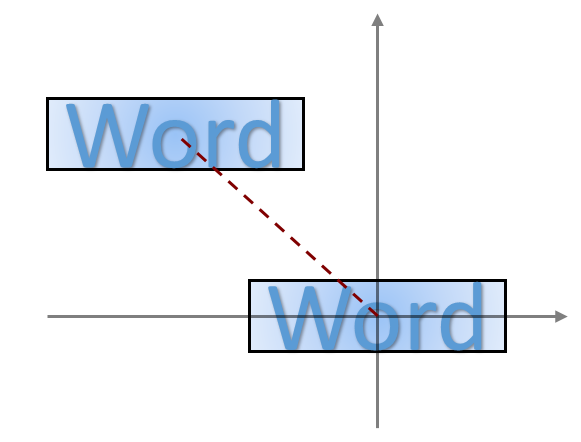
\includegraphics[scale=0.7]{img/wc_dinamiche/morph_4.png}}
\hspace{5mm}
\subfigure[]
{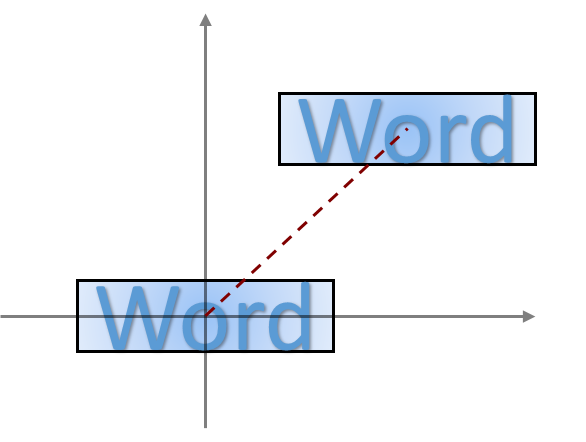
\includegraphics[scale=0.7]{img/wc_dinamiche/morph_1.png}}
\hspace{5mm}
\vspace{10mm}
\subfigure[]
{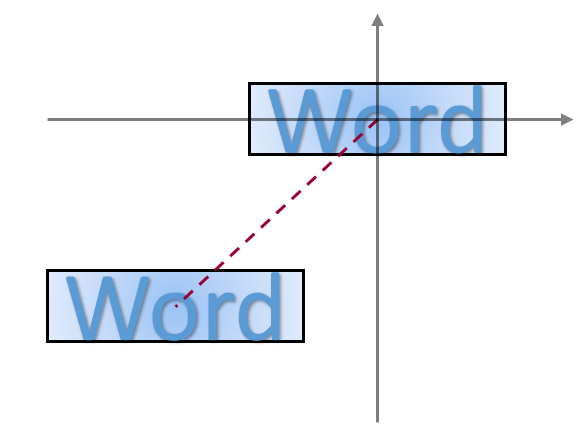
\includegraphics[scale=0.7]{img/wc_dinamiche/morph_3.png}}
\hspace{5mm}
\subfigure[]
{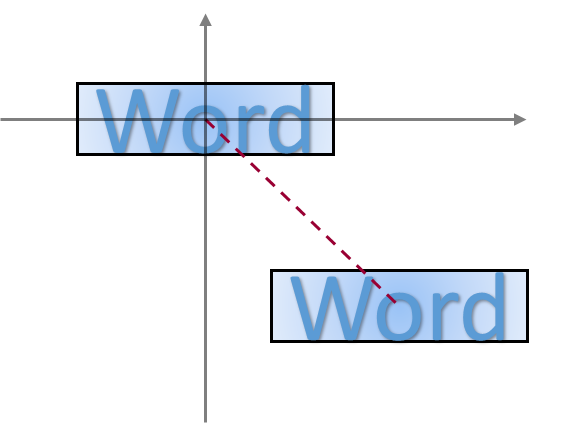
\includegraphics[scale=0.7]{img/wc_dinamiche/morph_2.png}}
\caption[Morphing delle parole comuni a $\Gamma_{i}^{k-1}$ e $\Gamma_{i}^{k}$.]{Morphing delle parole comuni a $\Gamma_{i}^{k-1}$ e $\Gamma_{i}^{k}$. Al centro c'� $\Gamma_{i}^{k-1}$, mentre $\Gamma_{i}^{k}$ pu� trovarsi in uno dei quattro quadranti.}
\label{fig:morphcommon}
\end{figure}
\end{enumerate}
Per quanto riguarda il colore delle parole, si considera il modello di colori RGB (Red, Green, Blue), secondo cui un'immagine pu� essere scomposta in tre colori principali, cio� rosso, verde e blu. Ogni colore � espresso da un intero compreso in $[0,255]$, che � l'intervallo che rappresenta lo spettro dei colori dal nero (valore pari a $0$) al bianco (valore pari a $255$). Ne segue quindi che ogni parola assume un colore dato dalla combinazione di tre interi. La trasformazione da un colore ad un altro viene gestito in modo indipendente per le tre componenti del colore. Dunque, le considerazioni che seguono valgono per ognuna delle componenti del colore.

Come sopra, siano dati due disegni consecutivi $\Gamma^{k-1}$ e $\Gamma^{k}$, intervallati da $N$ frame, e siano dati due interi $x$ e $y$, rappresentanti la stessa componente (rosso, verde o blu) di un colore, rispettivamente in $\Gamma^{k-1}$ e in $\Gamma^{k}$. Volendo raggiungere il valore di $y$ a partire da $x$, la variazione (incremento o decremento, a seconda dei casi) di colore ad ogni frame � pari a $\Delta(x,y) = \ceil[\bigg]{\dfrac{\vert x - y \vert}{N+1}} $. \\  Dunque, data una parola $w_{i}$, si hanno i seguenti tre casi:
\begin{enumerate}
\item $w_{i} \in C$: $w_{i}$ compare solo in $\Gamma^{k}$, con colore espresso dall'intero $y$. Poich� $w_{i}$ non � presente in $\Gamma^{k-1}$, si pu� assumere che, per raggiungere l'intero $y$, il valore $x$ di $w_{i}$ sia inizialmente pari a $255$, valore che rappresenta il bianco (che � lo sfondo della zona di disegno). In altre parole, ad ogni frame, si effettua un  decremento pari a $\Delta(x,y) = \ceil[\bigg]{\dfrac{x-y}{N+1}}$, dove $x=255$.
\item $w_{i} \in S$: $w_{i}$ compare solo in $\Gamma^{k-1}$, con  colore espresso dall'intero $x$. In maniera opposta al caso precedente, si parte da $x$ e si vuole raggiungere l'intero $255$. L'incremento, ad ogni frame, � $\Delta(x,y) = \ceil[\bigg]{\dfrac{y-x}{N+1}}$, dove $y=255$.
\item $w_{i} \in P$: $w_{i}$ compare in $\Gamma^{k-1}$ con colore dato dall'intero $x$ e in $\Gamma^{k}$ con colore dato dall'intero $y$. Per passare da $x$ a $y$, si considerano due casi:
\begin{itemize}
\item se $x<y$, allora l'incremento, ad ogni frame, � $\ceil[\bigg]{\dfrac{y\,-\,x}{N\,+\,1}}$;
\item se $x>y$, allora il decremento, ad ogni frame, � $\ceil[\bigg]{\dfrac{x\,-\,y}{N\,+\,1}}$;
\end{itemize}
\end{enumerate} 
Inoltre, poich� viene usata la parte intera superiore, la variazione minima di colore in ogni frame � pari ad $1$. Ci� significa che, una volta raggiunto il valore cercato (cio� $y$), il colore non varia pi�. 
%...

%%APPENDICI==============================================
% \appendix
% \input{appendiceA}
%...

%%BIBLIOGRAFIA============================================
\normalsize
\newpage
\bibliographystyle{unsrt}
\bibliography{bibliografia}

\end{document}
